%%%%%%%%%%%%%%%%%%%%%%%%%%%%%%%%%%%%%%%%%
% Short Sectioned Assignment
% LaTeX Template
% Version 1.0 (5/5/12)
%
% This template has been downloaded from:
% http://www.LaTeXTemplates.com
%
% Original author:
% Frits Wenneker (http://www.howtotex.com)
%
% License:
% CC BY-NC-SA 3.0 (http://creativecommons.org/licenses/by-nc-sa/3.0/)
%
%%%%%%%%%%%%%%%%%%%%%%%%%%%%%%%%%%%%%%%%%

%----------------------------------------------------------------------------------------
%	PACKAGES AND OTHER DOCUMENT CONFIGURATIONS
%----------------------------------------------------------------------------------------

\documentclass[paper=a4, fontsize=12pt]{scrartcl} % A4 paper and 11pt font size

\usepackage[T1]{fontenc} % Use 8-bit encoding that has 256 glyphs
\usepackage{fourier} % Use the Adobe Utopia font for the document - comment this line to return to the LaTeX default
\usepackage[english]{babel} % English language/hyphenation
\usepackage{amsmath,amsfonts,amsthm} % Math packages

\usepackage{graphicx}
\usepackage{extarrows}
\usepackage{amssymb}

\usepackage{lipsum} % Used for inserting dummy 'Lorem ipsum' text into the template

\usepackage{sectsty} % Allows customizing section commands
\allsectionsfont{\centering \normalfont\scshape} % Make all sections centered, the default font and small caps

\usepackage{fancyhdr} % Custom headers and footers
\pagestyle{fancyplain} % Makes all pages in the document conform to the custom headers and footers
\fancyhead{} % No page header - if you want one, create it in the same way as the footers below
\fancyfoot[L]{} % Empty left footer
\fancyfoot[C]{} % Empty center footer
\fancyfoot[R]{\thepage} % Page numbering for right footer
\renewcommand{\headrulewidth}{0pt} % Remove header underlines
\renewcommand{\footrulewidth}{0pt} % Remove footer underlines
\setlength{\headheight}{13.6pt} % Customize the height of the header

\numberwithin{equation}{section} % Number equations within sections (i.e. 1.1, 1.2, 2.1, 2.2 instead of 1, 2, 3, 4)
\numberwithin{figure}{section} % Number figures within sections (i.e. 1.1, 1.2, 2.1, 2.2 instead of 1, 2, 3, 4)
\numberwithin{table}{section} % Number tables within sections (i.e. 1.1, 1.2, 2.1, 2.2 instead of 1, 2, 3, 4)

\setlength\parindent{0pt} % Removes all indentation from paragraphs - comment this line for an assignment with lots of text

%----------------------------------------------------------------------------------------
%	TITLE SECTION
%----------------------------------------------------------------------------------------

\newcommand{\horrule}[1]{\rule{\linewidth}{#1}} % Create horizontal rule command with 1 argument of height

\title{	
\normalfont \normalsize 
\textsc{National Sun Yat-sen University, Department of Mathematics} \\ [25pt] % Your university, school and/or department name(s)
\horrule{0.5pt} \\[0.4cm] % Thin top horizontal rule
\huge Reliability Analysis Assignment 2 \\(personal)\\ % The assignment title
\horrule{2pt} \\[0.5cm] % Thick bottom horizontal rule
}

\author{Kuan-I Chung} % Your name

\date{\normalsize 2017.03.20} % Today's date or a custom date

\begin{document}

\maketitle % Print the title

%----------------------------------------------------------------------------------------
%	2.4
%----------------------------------------------------------------------------------------
2.4
\begin{itemize}

	\item[(a)]{
		\begin{equation*}
			f(t) = \frac{d}{dt}F(t) 	=  -exp\{-(\frac{t}{\eta})^\beta\}(-\beta(\frac{t}{\eta})^{\beta-1}\frac{1}{\eta})\\
						       	=  \frac{\beta}{\eta}(\frac{t}{\eta})^{\beta-1}exp\{ -(\frac{t}{\eta})^\beta\}
		\end{equation*}
	}
	
	\item[(b)]{
		\begin{equation*}
			h(t) 	= \frac{f(t)}{S(t)} = \frac{f(t)}{1-F(t)}\\
				= \frac{\frac{\beta}{\eta}(\frac{t}{\eta})^{\beta-1}exp\{ -(\frac{t}{\eta})^\beta\}}
					{1-(1-exp\{-(\frac{t}{\eta})^\beta \})} = \frac{\beta}{\eta}(\frac{t}{\eta})^{\beta-1}
		\end{equation*}
	}
	
	\item[(c)]{
		\
		\begin{figure}[h]
			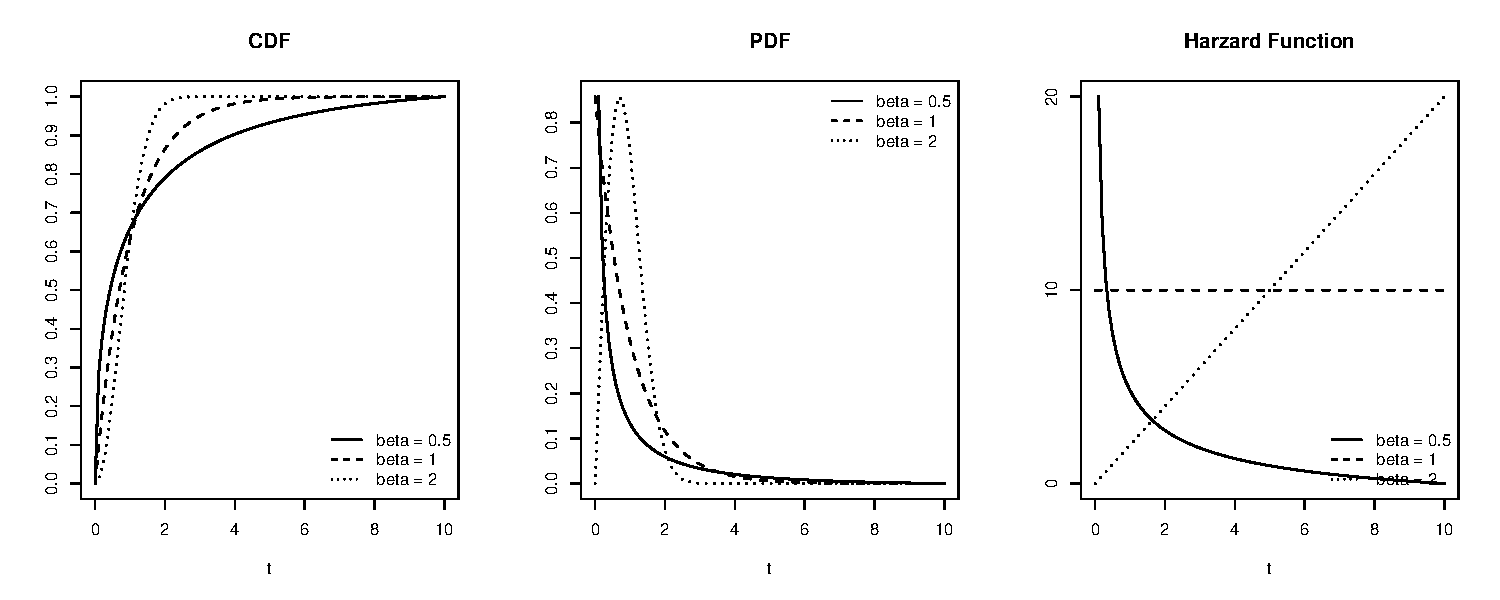
\includegraphics[width = 4.8 in]{2_4_c.pdf}
		\end{figure}
	}

\end{itemize}

%----------------------------------------------------------------------------------------
%	2.7
%----------------------------------------------------------------------------------------
2.7 \qquad $h(t) = 75 \cdot 10^{-9}\  \Rightarrow \ (75 \cdot 10^{-9})(20 \cdot 1500)(8760 \cdot 2) = 39.42\ \text{(units)} $\\

%----------------------------------------------------------------------------------------
%	2.13
%----------------------------------------------------------------------------------------
2.13 
\begin{itemize}
	\item[(i)] {
		Given $f(t)$
		\begin{align*}
			F(t) 	&= 	\int_0^t f(x) dx\\
			S(t) 	&= 	1 - F(t) = 1 - \int_0^t f(x) dx\\
			h(t) 	&=	\frac{f(t)}{1 - F(t)} = \frac{f(t)}{1 -  \int_0^t f(x) dx}\\
			H(t)	&=	-log\left(1-F(t)\right) = -log\left(1 -  \int_0^t f(x) dx \right)
		\end{align*}
	}
	\item[(ii)] {
		Given $F(t)$
		\begin{align*}
			f(t) 	&=	\frac{d}{dt} F(t)\\
			S(t)	&=	1-F(t)\\
			h(t)	&=	\frac{\frac{d}{dt}F(t)}{1-F(t)}\\
			H(t)	&=	-log\left(1-F(t)\right)
		\end{align*}
	}
	\item[(iii)] {
		Given $S(t)$
		\begin{align*}
			f(t)	&=	\frac{d}{dt}F(t) =\frac{d}{dt}(1-S(t))\\
			F(t)	&=	1-S(t)\\
			h(t)	&=	\frac{\frac{d}{dt}(1-S(t))}{S(t)}\\
			H(t)	&=	-log\left(S(t)\right)
		\end{align*}
	}
	\item[(iv)] {
		Given $h(t)$
		\begin{align*}
			H(t)	&=	\int_0^th(x) dx\\
			S(t)	&=	exp(-H(t)) = exp\left(-\int_0^th(x) dx\right)\\
			F(t)	&=	1-exp(-H(t)) = 1- exp\left(-\int_0^th(x) dx\right)\\
			f(t)	&=	\frac{d}{dt}F(t) = exp\left(-\int_0^th(x) dx\right)\cdot h(t)
		\end{align*}
	}
	\item[(v)] {
		Given $H(t)$
		\begin{align*}
			h(t) 	&= 	\frac{d}{dt} H(t)\\
			S(t)	&=	exp\{-H(t)\}\\
			F(t)	&=	1 - exp\{-H(t)\}\\
			f(t)	&=	\frac{d}{dt} F(t) = exp\{-H(t)\}\cdot \left(H(t) \right)
		\end{align*}
	}
\end{itemize}

%----------------------------------------------------------------------------------------
%	2.14
%----------------------------------------------------------------------------------------
2.14
\begin{itemize}
	\item[(a)]{
		\begin{align*}
				&	Pr(t_{i-1} < T \leq t_i \vert T>t_{i-1})\\
			=	&	\frac{Pr(t_{i-1} < T \leq t_i ,\ T>t_{i-1})}{Pr(T>t_{i-1})}
			=		\frac{Pr(t_{i-1} < T \leq t_i)}{1-Pr(T>t_{i-1}))}\\
			=	&	\frac{F(t_i)-F(t_{i-1})}{1-F(t_{i-1})} = \frac{\pi_i}{S(t_{i-1})}
		\end{align*}
	}
	
	\item[(b)]{
		\begin{itemize}
			\item[(i)]{
				\begin{align*}
					\pi_1 	&=	Pr(t_0 < T \leq t_1) = \frac{Pr(t_0 < T \leq t_1, T>t_0)}{Pr(T>t_0)} Pr(T>t_0)\\
							&=	Pr(t_0 < T \leq t_1 \vert T>t_0)\cdot 1 = p_1
				\end{align*}
			}
			
			\item[(ii)]{
				\begin{align*}
					\pi_i 		&= 	Pr(t_{i-1} < T \leq t_i) = \frac{Pr(t_{i-1} < T \leq t_i)}{Pr(T>t_{i-1})}Pr(T>t_{i-1})\\
							&=	p_i \cdot  \frac{Pr(T>t_{i-1})}{Pr(T>t_{i-2})} \cdot \frac{Pr(T>t_{i-2})}{Pr(T>t_{i-3})} 
								\cdots \frac{Pr(T>t_{i})}{Pr(T>t_{0})} \cdot Pr(T>t_{0})\\
							&=	p_i \cdot \frac{Pr(T>t_{i-2})-Pr(t_{i-2}<T\leq t_{i-1})}{Pr(T>t_{i-2})} \cdots 
								\frac{Pr(T>t_{1})-Pr(t_{1}<T\leq t_{2})}{Pr(T>t_{1})}\cdot Pr(T>t_{0})\\
							&=	p_i\cdot (1-p_{i-1})\cdot (1-p_{i-1})\cdots(1-p_1) \cdot 1 
							  = 	p_i \prod_{j=1}^{i-1}(1-p_j) \\
							&	\forall i=1,2,\dots , m
				\end{align*}
			}
			
			\item[(iii)]{
				\begin{align*}
					\pi_{m+1}	&=	p_{m+1} \prod_{j=1}^{m+1-1}(1-p_j) \\
							&=	\frac{Pr(t_m<T\leq t_{m+1})}{Pr(T>t_m)}\prod_{j=1}^{m}(1-p_j)
							\xlongequal{t_{m+1} \rightarrow \infty}	\frac{Pr(T>t_m)}{Pr(T>t_m)}\prod_{j=1}^{m}(1-p_j)\\
							&=	\prod_{j=1}^{m}(1-p_j)\\
				\end{align*}
			}
		\end{itemize}
	}
	
	\item[(c)]{
		\begin{align*}
					& 	p_i = \frac{F(t_i)-F(t_{i-1})}{1-F(t_{i-1})} = \frac{\pi_i}{S(t_{i-1})}\\
			\because 	&	\pi_i>0 \quad \forall i = 1, \dots, m+1\\
			\therefore 	&	S(t_{i})>0 \quad i.e. F(t_i)<1 \quad \forall i = 1, \dots, m+1\\
		 	\therefore 	&	p_i \neq 0 \land p_i \neq 1\\
			\because 	&	p_i = Pr(t_{i-1}<T\leq t_{i} \vert T>t_{i-1}) \\
			\therefore 	&	0\leq p_i \leq1\\
			\Rightarrow&	0<p_i<1 \quad \forall i = 1, \dots, m+1
		\end{align*}
	}
	
	\item[(d)]{
		By the statement (i), (ii) and (iii) in (b),
		\begin{align*}
			\pi_i 		&= 	Pr(t_{i-1} < T \leq t_i) = \frac{Pr(t_{i-1} < T \leq t_i)}{Pr(T>t_{i-1})}Pr(T>t_{i-1})\\
					&=	p_i \cdot S(t_{i-1}) =	p_i \prod_{j=1}^{i-1}(1-p_j)\quad \forall i = 1, \dots, m+1\\
					&\Rightarrow S(t_i) = \prod_{j=1}^{i}(1-p_j) \quad \forall i = 1, \dots, m+1
		\end{align*}
	}
\end{itemize}


%----------------------------------------------------------------------------------------
%	2.16
%----------------------------------------------------------------------------------------
2.16
\begin{align*}
	\because	&	H(T) =-log(1-F(T))\\
			&	Pr(H(T) \leq t) = Pr(-log(1-F(T)) \leq t) \\
	=		&	Pr(1-F(T) \leq e^{-t}) = Pr(F(T) \geq 1- e^{-t} )\\
	=		&	e^{-t}\\
	\Rightarrow&	H(t) \ \text{follows an exponential distribution.}
	\end{align*}

%------------------------------------------------
\end{document}